\subsection{Kiểm chứng thanh toán VNPay}
Unit test kiểm HMAC bằng vector RFC 4231, chuẩn hóa khoảng trắng/ký tự đặc biệt, callback sửa tiền/trường trùng, giờ GMT+7 và chữ ký QueryDr. API integration dùng gateway giả lập có chữ ký test cùng PostgreSQL riêng để chủ động tạo callback lặp, trễ và lỗi giữa transaction.

\begin{table}[htbp]\centering\small
\begin{tabularx}{\linewidth}{|p{.13\linewidth}|X|}\hline
\textbf{Mã} & \textbf{Hành vi cần chứng minh}\\\hline
PAY-01 & Backend quyết định amount/merchant; cùng key hoặc key mới tái dùng mã còn hiệu lực.\\\hline
PAY-02 & IPN thành công đồng thời chỉ có một Payment và một lần cộng điểm.\\\hline
PAY-03 & Return hợp lệ chỉ redirect, không tự chuyển Order sang PAID.\\\hline
PAY-04 & Chữ ký, merchant hoặc amount sai không cập nhật đơn.\\\hline
PAY-05 & Timeout tra cứu không tự đánh dấu thất bại; retry sau hết hạn giữ đủ lịch sử attempt.\\\hline
PAY-06 & Hai khoản thu cùng đơn chỉ một khoản áp dụng, khoản dư có hồ sơ xử lý.\\\hline
PAY-07 & Khách không xem giao dịch người khác/gọi API staff; bật VNPay thì API mock bị chặn.\\\hline
PAY-08 & Thất bại đến sau thành công không hạ PAID; lỗi cộng điểm rollback, IPN retry có thể xử lý lại.\\\hline
\end{tabularx}\caption{Các ca kiểm chứng chữ ký, vòng đời và tính nhất quán thanh toán}
\end{table}

Các ca tương ứng nằm tại \path{src/payments/vnpay.crypto.spec.ts}, \path{test/vnpay.e2e-spec.ts} và bộ retry/đổi món. Các kiểm tra hạn QR và IPN sau deadline liên kết với KHO-12 đến KHO-14. Số liệu bộ hồi quy đã ghi tại mục~\ref{sec:inventory-tests}; không cộng lại thành một kết quả chạy mới hoặc diễn giải gateway giả lập là giao dịch tiền thật.

\begin{figure}[htbp]\centering
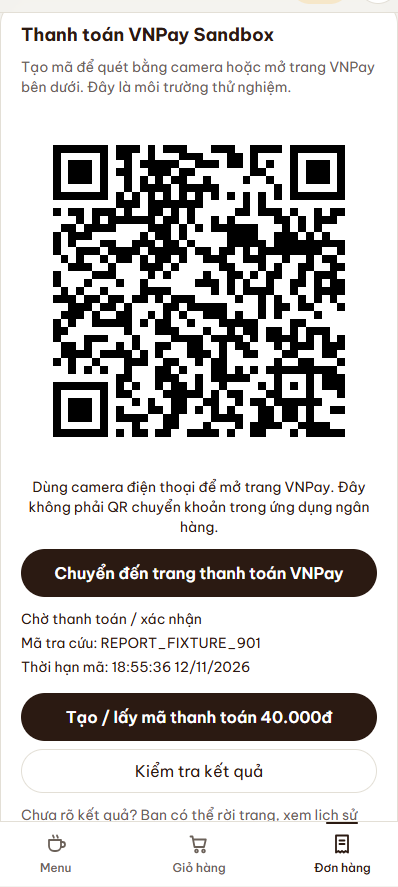
\includegraphics[width=.32\linewidth,height=.40\textheight,keepaspectratio]{assets/vnpay/payment-ui-fixture.png}
\caption{Màn hình QR và nút mở trang VNPay; ảnh UI dùng API fixture với tham chiếu thử}
\end{figure}
